\documentclass[12pt,a4paper]{report} % Ajout de la taille de police 12pt pour le confort

% --- PACKAGES ---
\usepackage[utf8]{inputenc}
\usepackage[T1]{fontenc}
\usepackage[french]{babel}
\usepackage{titlesec}
\usepackage{tocloft}
\usepackage{graphicx}
\usepackage{float}
\usepackage[colorlinks=true, linkcolor=blue, citecolor=green]{hyperref}
\usepackage{minted} % Nécessite -shell-escape lors de la compilation
\usepackage{wrapfig}
\usepackage{array}
\usepackage{amsmath, amssymb, amsthm}
\usepackage{mdframed}
\usepackage[a4paper, left=2.5cm, right=2.5cm, top=2.5cm, bottom=2.5cm]{geometry}
\usepackage{background}
\usepackage{lipsum} % À retirer à la fin

% --- ENVIRONNEMENTS MATHÉMATIQUES ---
\newtheorem{theorem}{Théorème}
\newtheorem{definition}{Définition}
\newtheorem{example}{Exemple}
\newtheorem{property}{Propriété}
\newmdtheoremenv{boxedproperty}{Propriété}[section]

% --- CONFIGURATION DU LOGO DE FOND (INSA) ---
\backgroundsetup{
scale=1, angle=0, opacity=1, color=black,
contents={\begin{tikzpicture}[remember picture,overlay]
\node at ([xshift=-0.8in,yshift=0.8in] current page.south east) 
{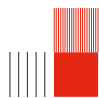
\includegraphics[scale=0.8]{images/pattern.png}}; 
\end{tikzpicture}}
}

% --- MISE EN FORME DES TITRES ---
\titleformat{\chapter}[display]
  {\normalfont\huge\bfseries}{\chaptertitlename\ \thechapter}{10pt}{\Huge}
\titleformat{\section}
  {\normalfont\Large\bfseries}{\thesection}{1em}{}
\titleformat{\subsection}
  {\normalfont\large\bfseries}{\thesubsection}{1em}{}

% --- CONFIGURATION TABLE DES MATIÈRES ---
\renewcommand{\cftchapfont}{\bfseries}
\renewcommand{\contentsname}{Table des matières}

% --- DÉBUT DU DOCUMENT ---
\begin{document}

% --- PAGE DE TITRE ---
\begin{titlepage}
    \centering
    \noindent 
    \begin{minipage}{0.45\textwidth}
        
\includegraphics[width=0.8\linewidth]{images/logo_INSA.png} 
    \end{minipage}%
    \hfill 
    \begin{minipage}{0.45\textwidth}
        \flushright 
        
\includegraphics[width=0.8\linewidth]{images/tescan_logo.png} 
    \end{minipage}

    \vspace*{2cm} 
    {\Huge\bfseries Rapport de Projet Multidisciplinaire \par}
    \vspace{1cm}
    {\huge Modélisation du Quadrupôle d'Okayama par BEM \par}
    \vspace{0.4cm}
    {\large (\textit{Boundary Element Method}) \par}
    \vspace{2cm}

    {\Large \textbf{Zoé \textsc{Nonon} --- Louise \textsc{Lammertyn}} \par}
    \vspace{0.2cm}
    {\large $4^{\text{ème}}$ année Génie Physique \par}
    
    \vspace{2.5cm}

    {\large \textbf{Tuteurs :}} \par
    \vspace{0.5cm}
    {\large
    \begin{tabular}{l}
        Florent \textsc{Houdellier} \\
        Lucile \textsc{Berdoux Durieux} \\
        Jean-Baptiste \textsc{Mellier} \\
        Pier-Francesco \textsc{Fazzini}
    \end{tabular}
    } \par
    
    \vfill 
    {\large Année universitaire 2025-2026 \par}
    \vspace{0.8cm}
    {\Large \textbf{Institut National des Sciences Appliquées de Toulouse} \par}
    \vspace{0.5cm}
    {\large \today \par}
\end{titlepage}

% --- REMERCIEMENTS ---
\chapter*{Remerciements}
\addcontentsline{toc}{chapter}{Remerciements}
Nous tenons à remercier nos tuteurs pour leur accompagnement...

% --- SOMMAIRE ---
\tableofcontents
\newpage

% --- CORPS DU RAPPORT (Votre plan spécifique) ---

\chapter{Contexte et objectifs du projet}
\section{Principe de l’optique de particules chargées}
\section{État de l’art de la simulation numérique}
\section{Objectifs}

\chapter{Travail réalisé}
\section{Formation OPC}
\subsection{Librairie BEMPP}
\subsection{Prise en main BEM}

\section{Cas du Quadrupôle}


[Image of quadrupole magnetic field lines]


\section{Décomposition multipolaire}

\section{Calcul des trajectoires paraxiales}

\section{Calcul des aberrations de Seidel}

\chapter{Récapitulatif et perspectives}
\section{Récapitulatif}
\section{Perspectives}

\chapter*{Conclusion}
\addcontentsline{toc}{chapter}{Conclusion}
Bilan du projet...

% --- LISTES ET BIBLIO ---
\newpage
\listoffigures
\addcontentsline{toc}{chapter}{Table des figures}

\listoftables
\addcontentsline{toc}{chapter}{Table des tableaux}

\newpage
\bibliographystyle{plain}
\bibliography{references}
\addcontentsline{toc}{chapter}{Références}

\end{document}